
% This LaTeX was auto-generated from MATLAB code.
% To make changes, update the MATLAB code and republish this document.

\documentclass{article}
\usepackage{graphicx}
\usepackage{color}

\sloppy
\definecolor{lightgray}{gray}{0.5}
\setlength{\parindent}{0pt}

\begin{document}

    
    \begin{verbatim}
n=[25,50,100];
dimN=size(n,2);
theta=1.2;
Legend=cell(dimN,1);

Counter=1;
figure
while Counter<=dimN
    Variables=zeros(n(Counter),3);
    Variables(:,1)=1:n(Counter);
    Variables(:,2)=rand(n(Counter),1);
    Variables(:,3)=-log(1-Variables(:,2))/theta;
    % disp(Variables)
    %Produces a latex table
    %latex(sym(vpa(Variables)))
    Max=log(2)*sum(Variables(:,3))/n(Counter);
    disp(Max)

    %Plots the log likelihood function
    m=linspace(0,5);
    y=loglike(Variables(:,3),m,n(Counter));
    plot(m,y)
    hold on
    Legend{Counter,1}=strcat('n=',num2str(n(Counter)));
    Counter=Counter+1;
end
xlabel("m")
ylabel("Log Likelihood function")
legend(Legend)
print('Image_3_4','-depsc')



%This calculates the log likelihood using the data x plotted against m
function answer=loglike(x,m,n)
    count=1;
    answer=1;
    while count<=n
        answer=answer.*g(x(count),m);
        count=count+1;
    end
    answer=log(answer);
end

%This is the p.d.f paramterised in terms of m
function answer=g(x,m)
    answer=log(2)./(m.*2.^(x./m));
end
\end{verbatim}

        \color{lightgray} \begin{verbatim}         0.639380887448366

         0.479387398667443

         0.526784599466113

\end{verbatim} \color{black}
    
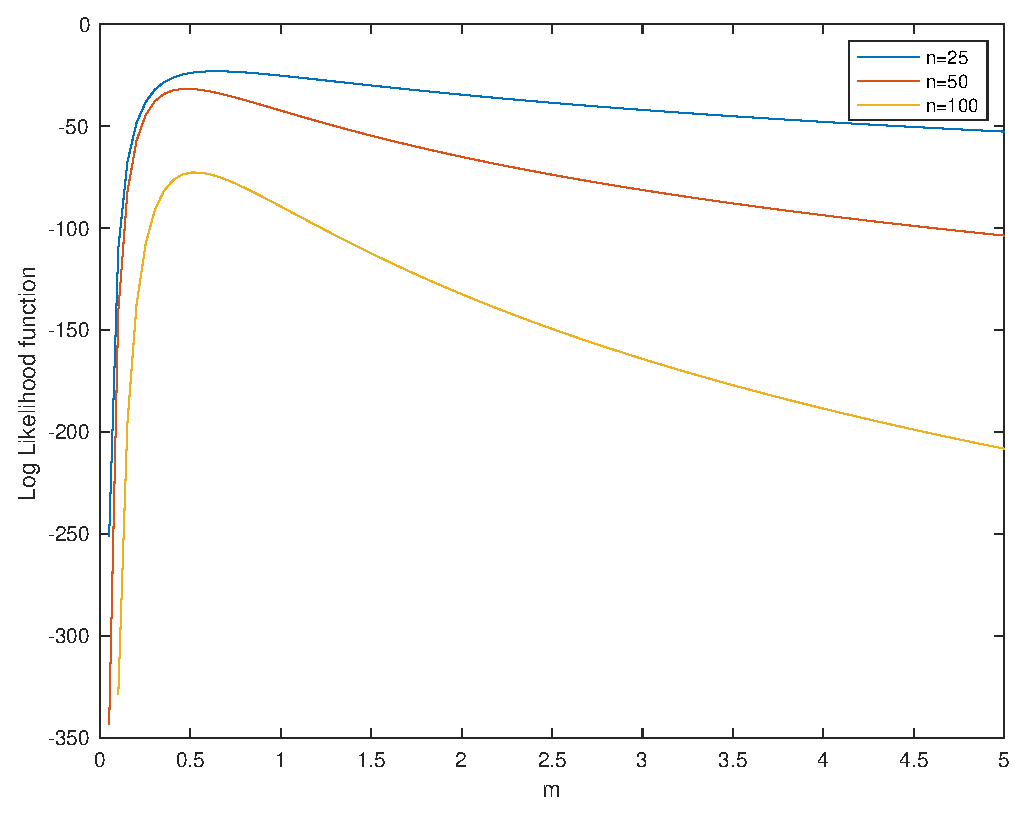
\includegraphics [width=4in]{Code_2_1_01.eps}



\end{document}
    
